\section{Chaotisches Verhalten}
Wie im vorherigen Kapitel angedeutet, wurde mithilfe der Gleichungen eine Simulation erstellt,
um das chaotische Verhalten näher zu analysieren.
Diese Simulation wurde von Alex Krieg, einem Studenten der <<Fachhochschule OST>>, entwickelt.
Die daraus gewonnenen Erkenntnisse werden in diesem Abschnitt erläutert.

\subsection{Physikalisches Chaos}
In der Physik wird das Chaos als aperiodisches Langzeitverhalten in einem deterministischen
System bezeichnet, mit empfindlicher Abhängigkeit der Anfangsbedingungen.
Aperiodisches Langzeitverhalten bedeutet, wenn sich das System nach langer zeitlicher Betrachtung
nicht periodisch wird.
Das einfache Pendel weist ein periodisches Langzeitverhalten auf,
denn es schwingt immer im gleichen Muster.
Deterministisch heisst, dass das Verhalten des Systems vorherbestimmbar ist.
Dies mag zunächst verwirrend erscheinen, da chaotisches Verhalten grundsätzlich nicht
berechenbar ist.
Was aber gemeint ist, man kann vorhersagen ob das System in einen chaotischen Zustand 
verfällt oder stabil bleibt.

\subsection{Simulationsanalyse}
Im ersten Experiment wollen wir uns ansehen wie der Trajektor eines Pendels aussieht,
welcher aus der horizontalen Lage bzw. Anfangsbedingung 90° startet.
(siehe Abbildung \ref{fig:pendel_bei_90})
Beim Wiederholen dieses Experiment lässt sich feststellen, dass für exakt dieselben Anfangsbedingungen
das gleiche Ergebnis resultiert und daher deterministisch ist.
\begin{figure}
    \centering
    \begin{minipage}{0.45\textwidth}
        \centering
        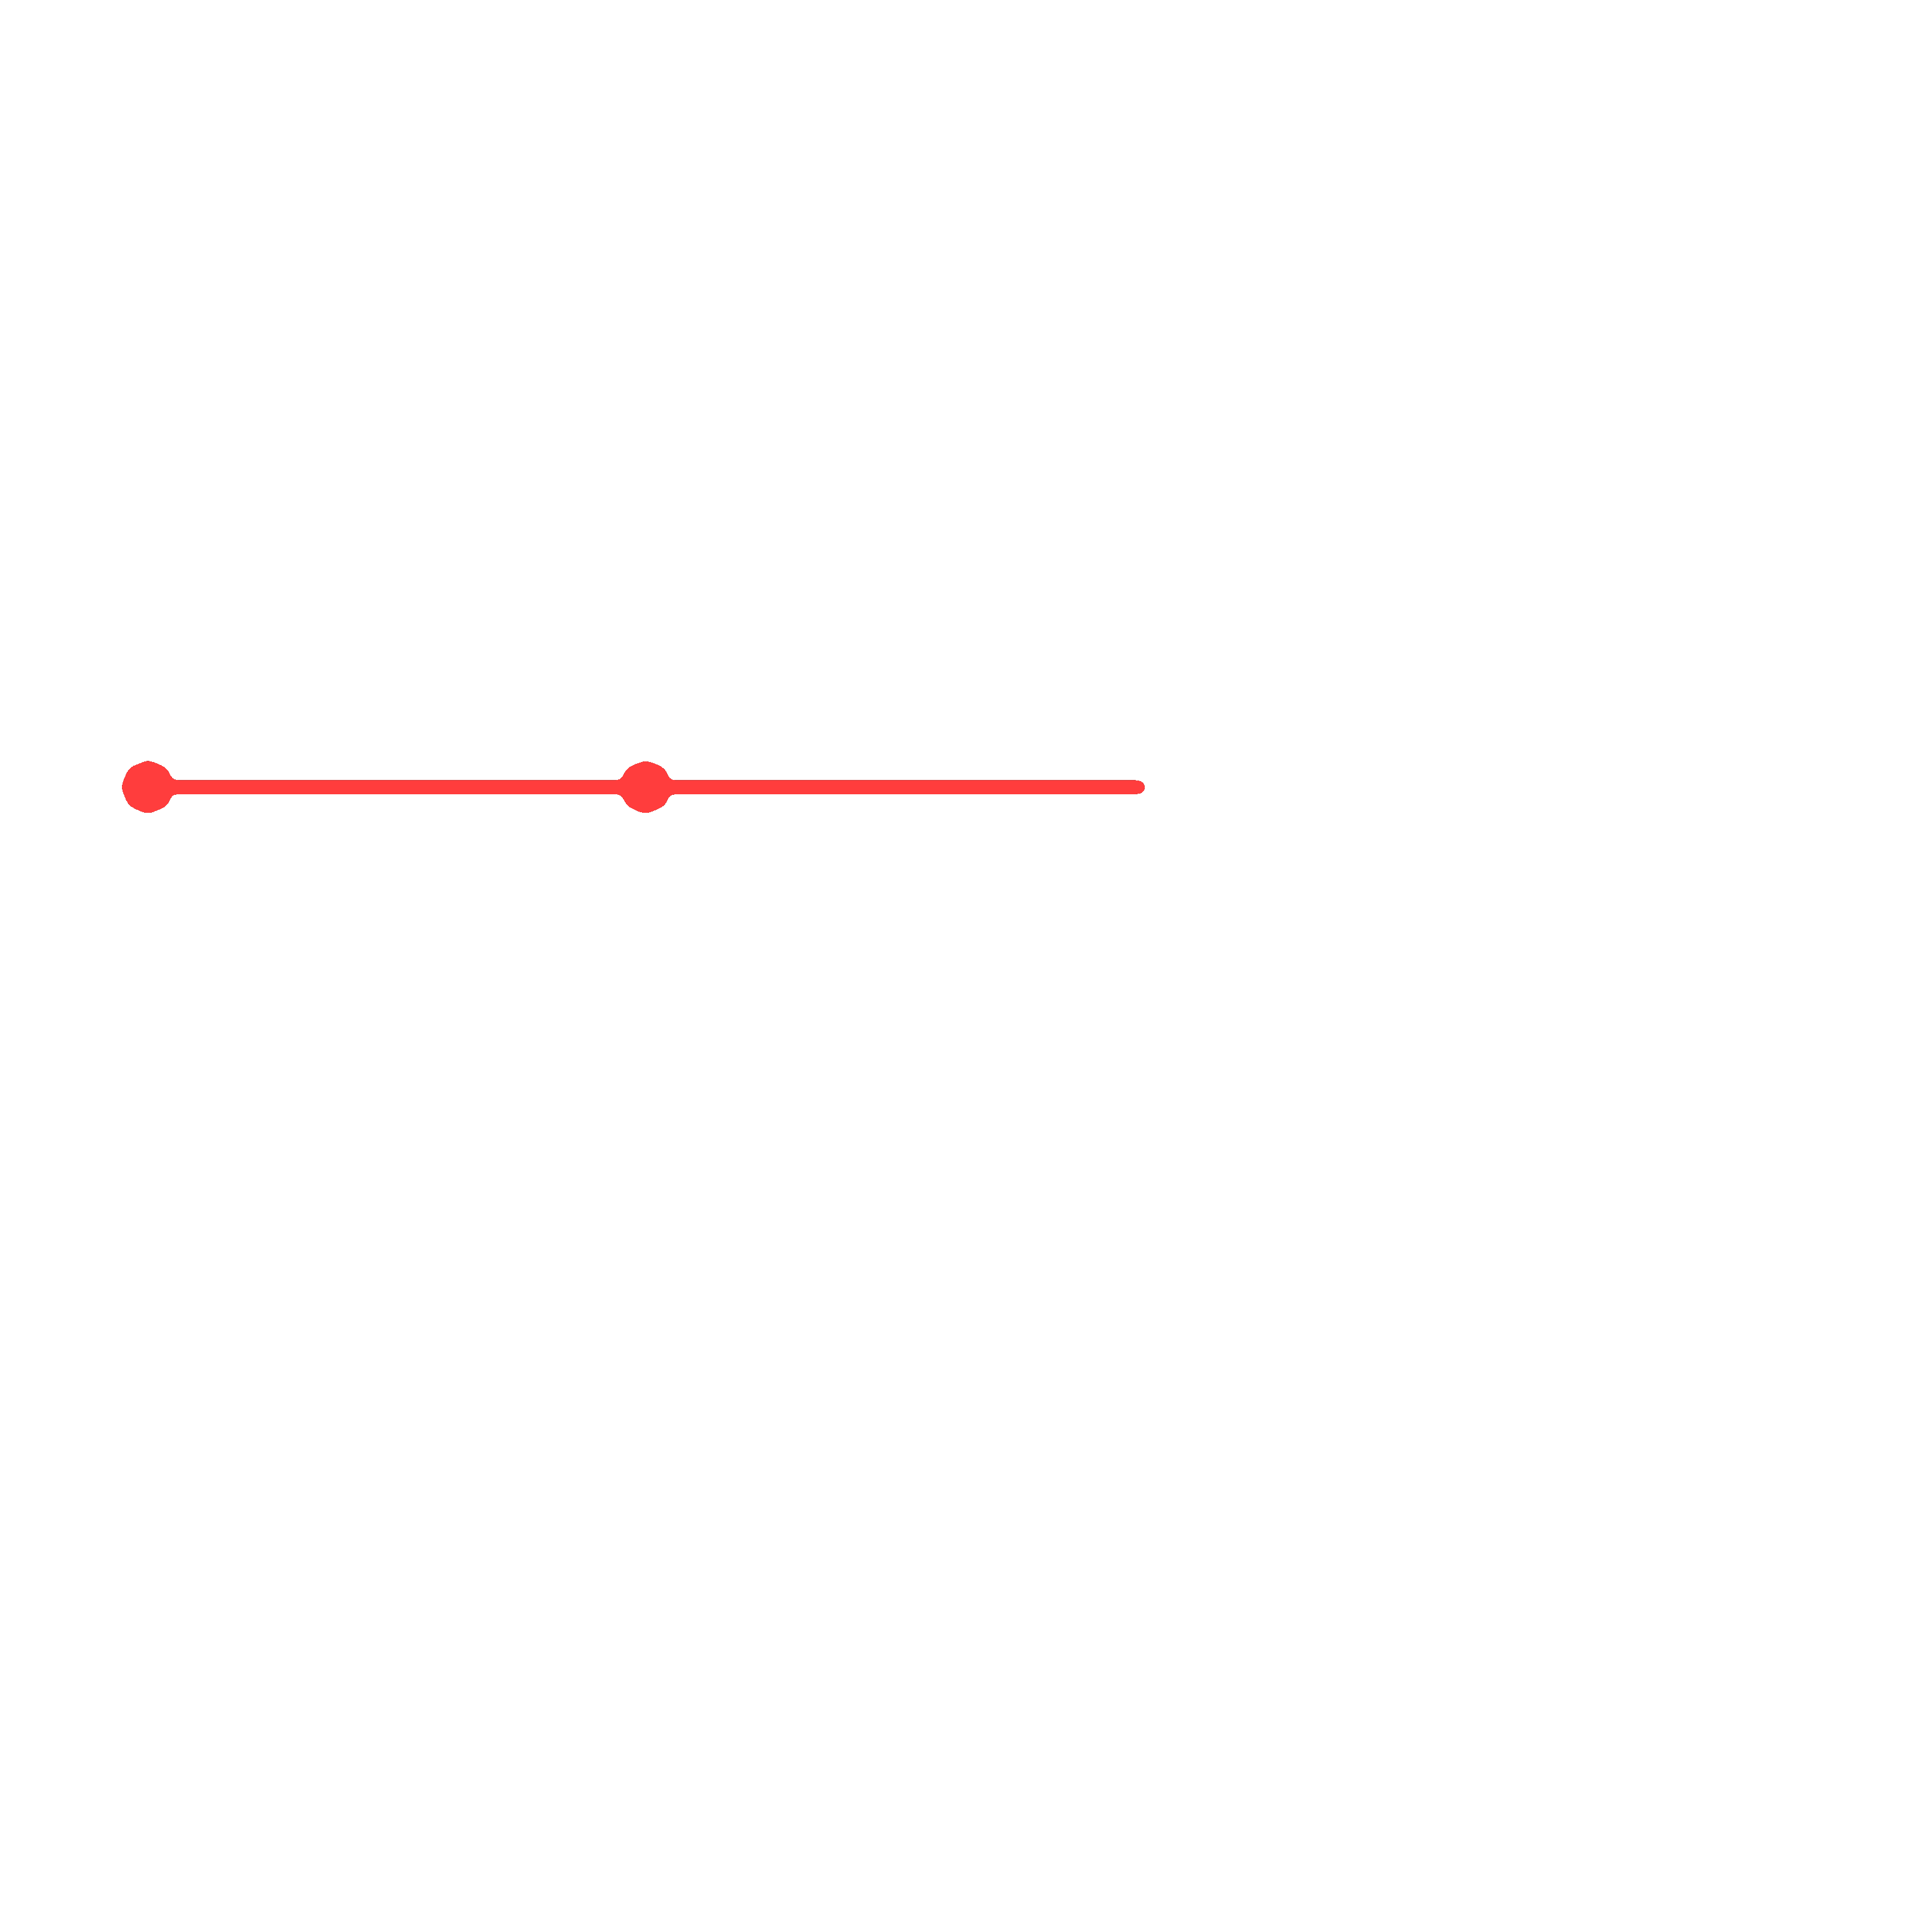
\includegraphics[width=\textwidth]{papers/doppelpendel/images/pendel_stand_90.png}
    \end{minipage}
    \hfill
    \begin{minipage}{0.45\textwidth}
        \centering
        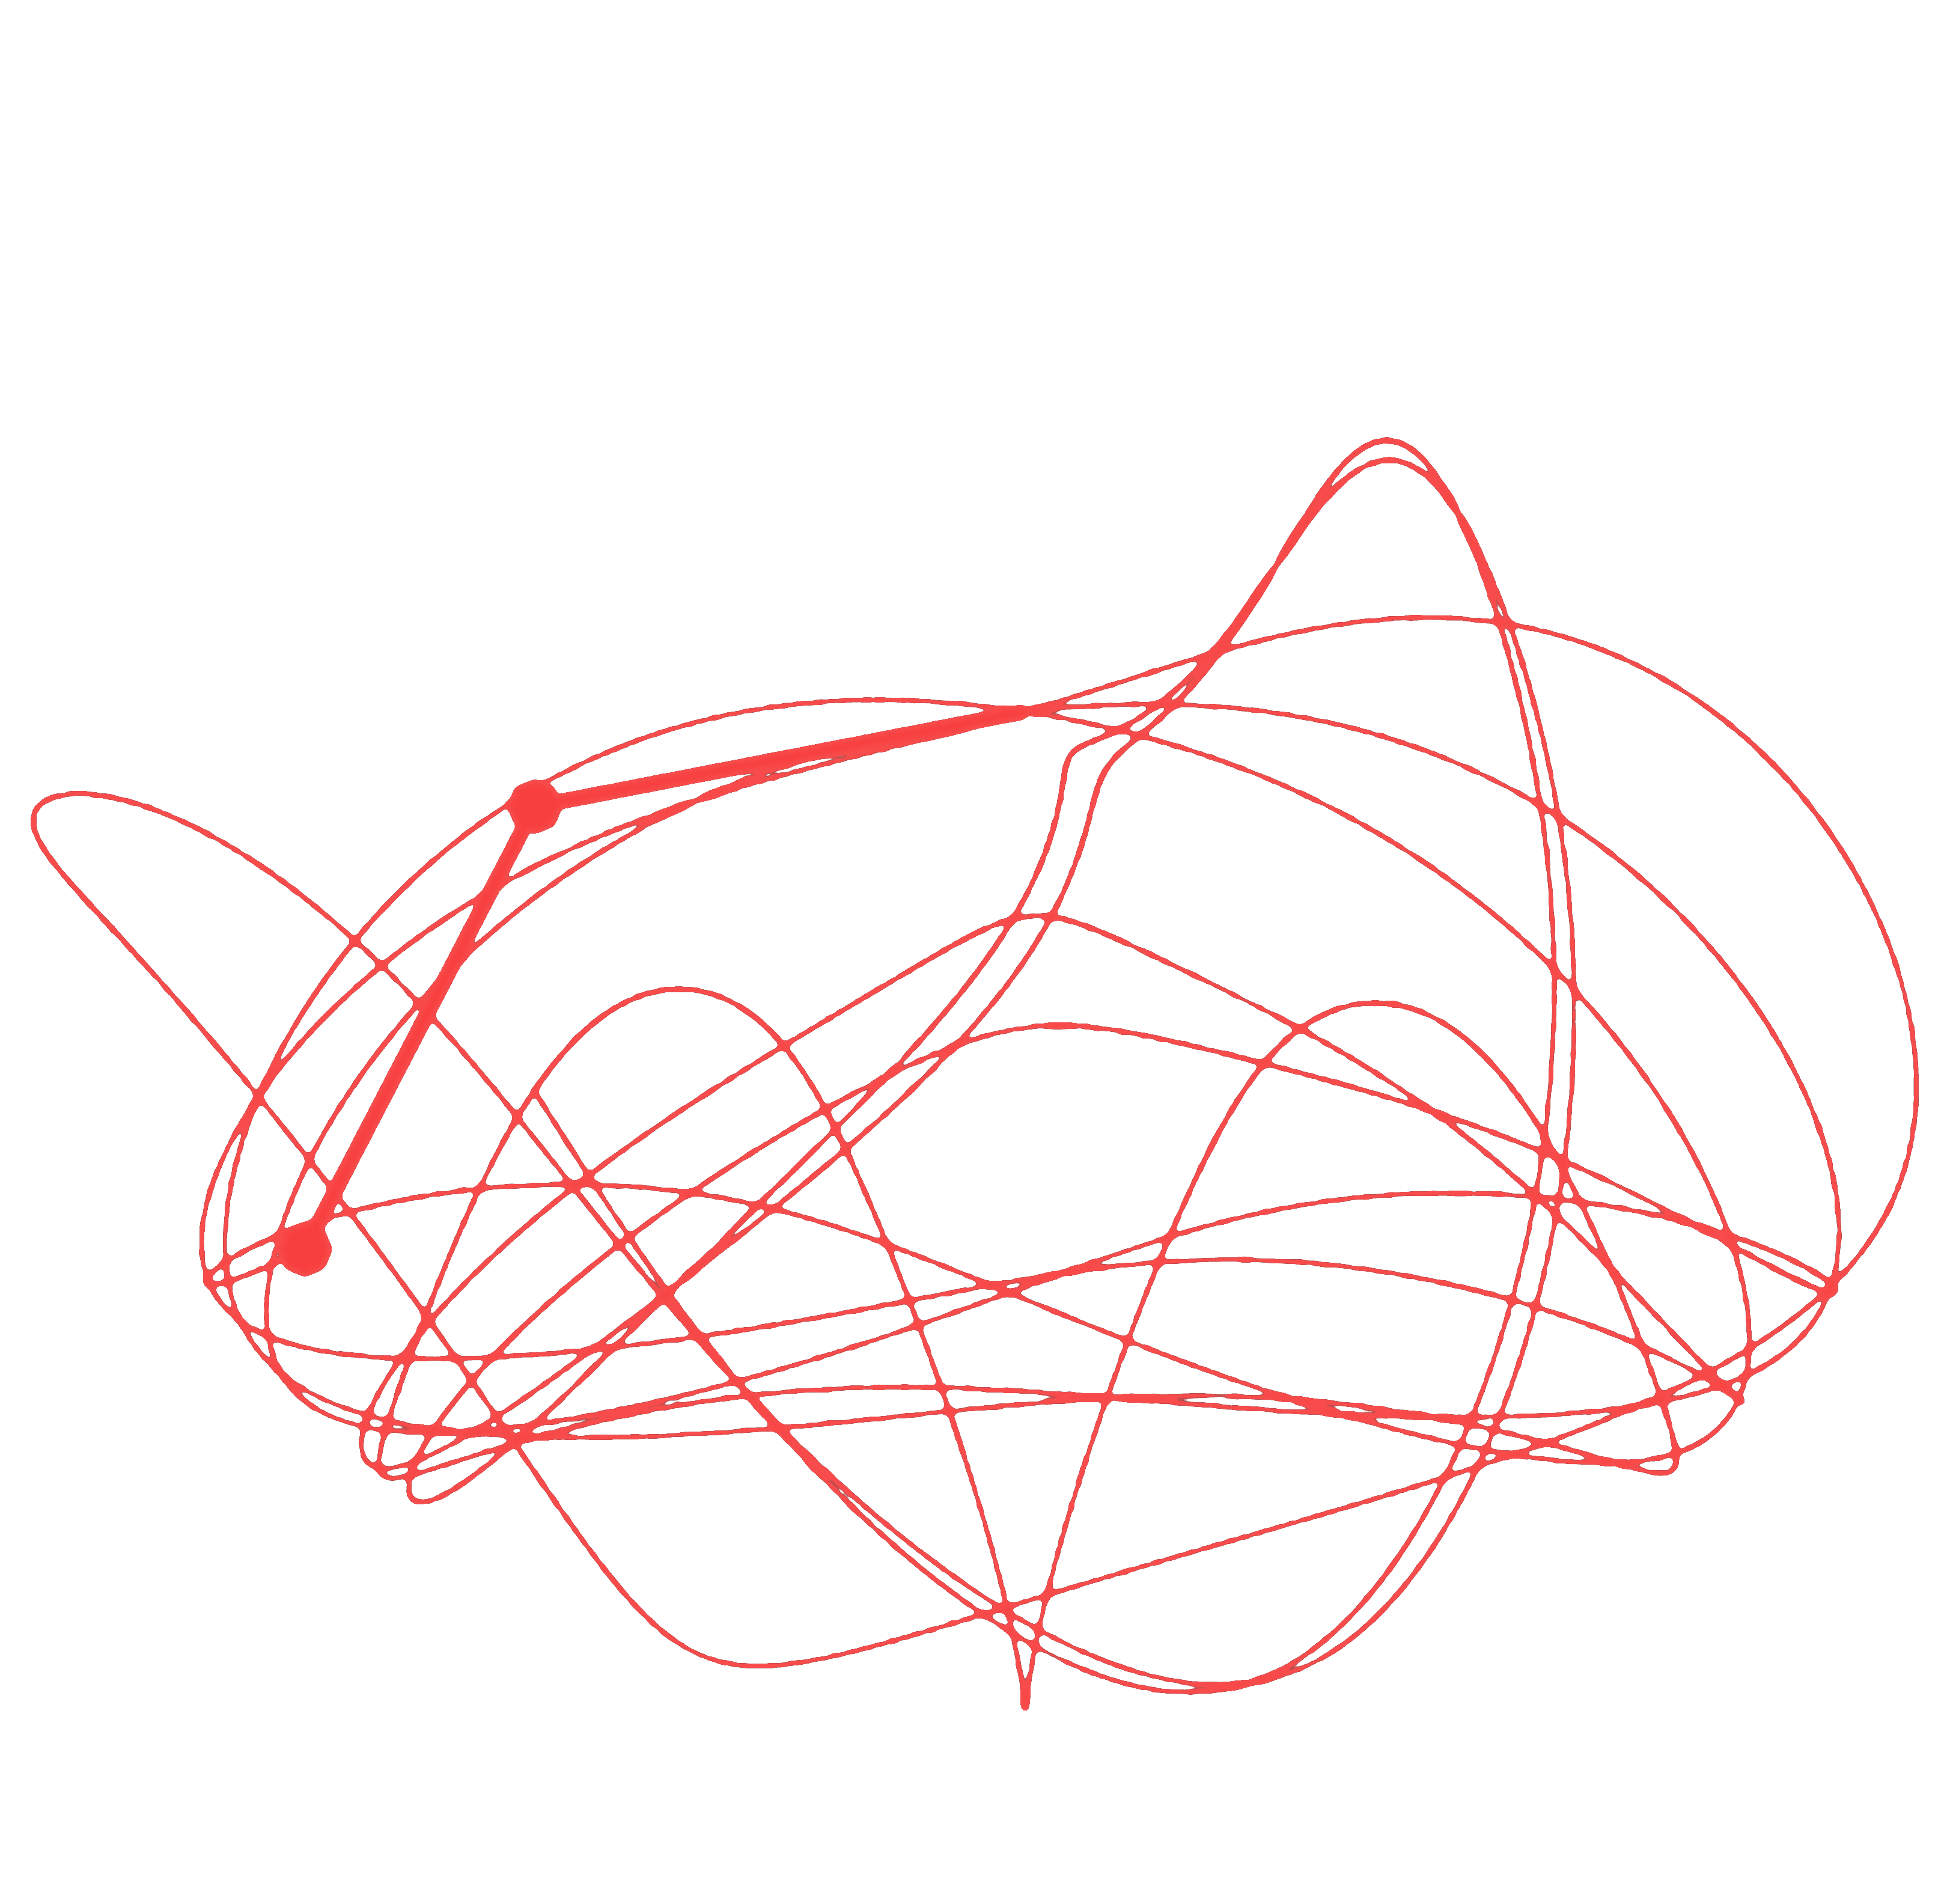
\includegraphics[width=\textwidth]{papers/doppelpendel/images/pendel_spur_90.png}
    \end{minipage}
    \caption{Pendel mit der Anfangsbedinung 90°.}
    \label{fig:pendel_bei_90}
\end{figure}

Im zweiten Experiment (Abbildung \ref{fig:pendel_bei_weniger_90}), wurde die vorherige
Anfangsbedingung marginal verändert.
Die beiden Winkel wurden um ca. Zehntel Grad verringert.
Nichtsdestotrotz lässt sich am Resultat nichts wiedererkennen.
\begin{figure}
    \centering
    \begin{minipage}{0.45\textwidth}
        \centering
        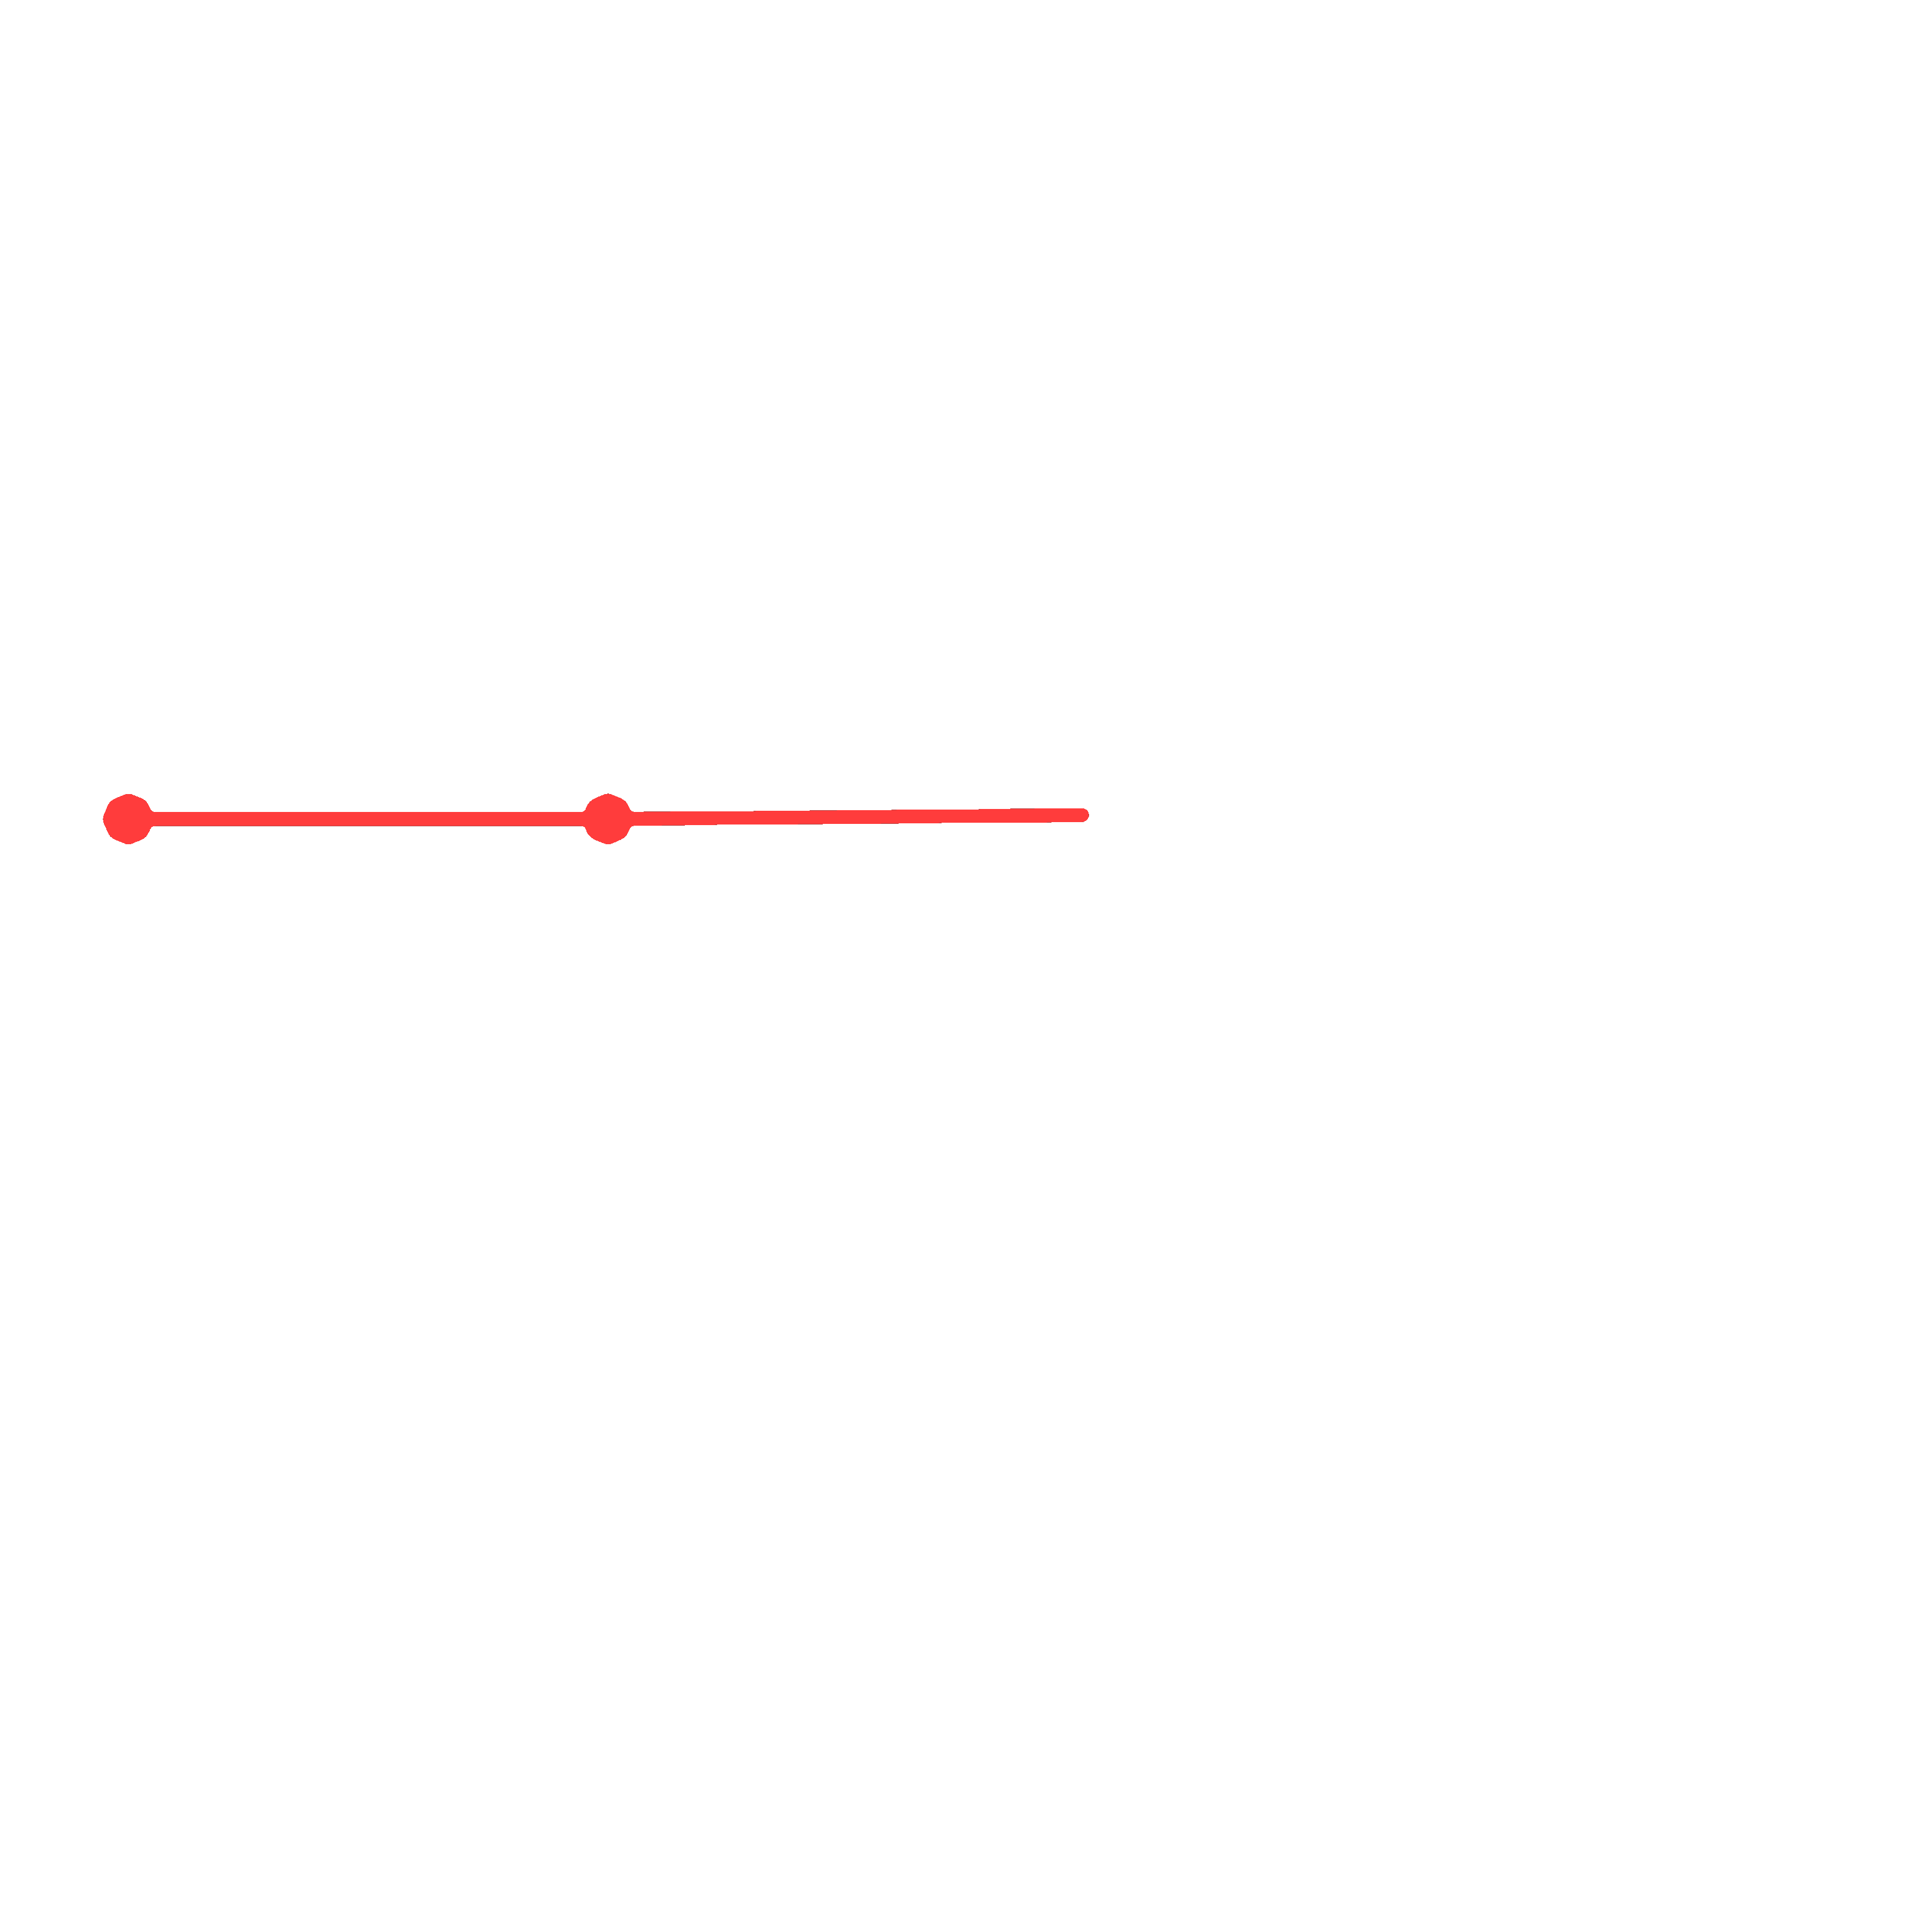
\includegraphics[width=\textwidth]{papers/doppelpendel/images/pendel_stand_kleiner_90.png}
    \end{minipage}
    \hfill
    \begin{minipage}{0.45\textwidth}
        \centering
        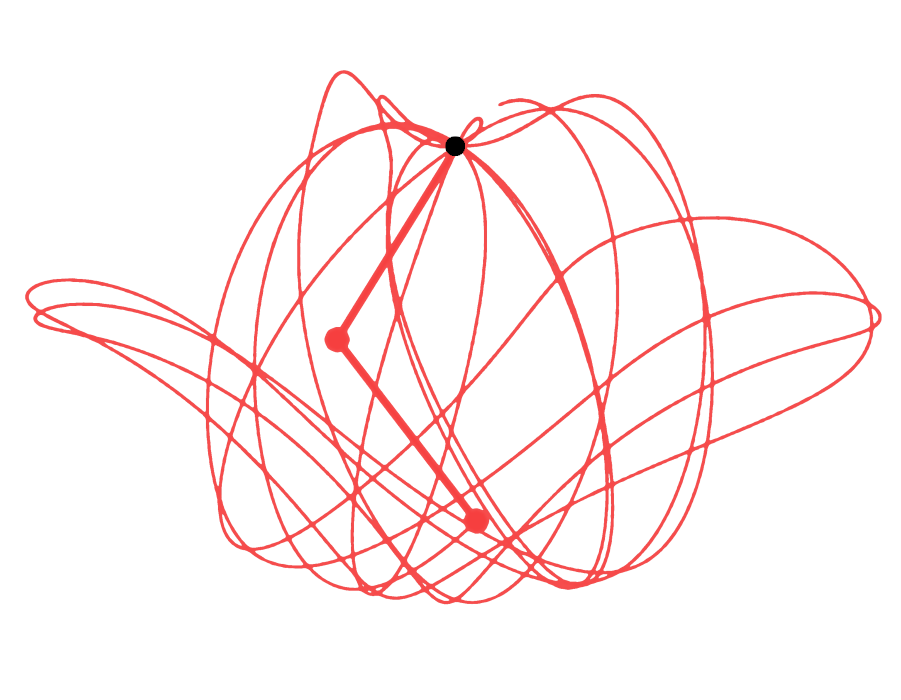
\includegraphics[width=\textwidth]{papers/doppelpendel/images/pendel_spur_kleiner_90.png}
    \end{minipage}
    \caption{Anfangsbedingung der Winkel ist kaum sichtbar kleiner als 90°.}
    \label{fig:pendel_bei_weniger_90}
\end{figure}

Im letzten Experiment (Abbildung \ref{fig:pendel_nichtchaotisch}) wird gezeigt,
wie das Pendel bei kleineren Winkeln nicht chaotisch wird.
Es lässt bereits vermuten, dass die Pendel mit hoher potentieller Energie eine stärkere Tendenz haben,
in den chaotischen Zustand überzugehen.
Das zeigen auch die Trajektoren aus diesen Versuchen.
\begin{figure}
    \centering
    \begin{minipage}{0.45\textwidth}
        \centering
        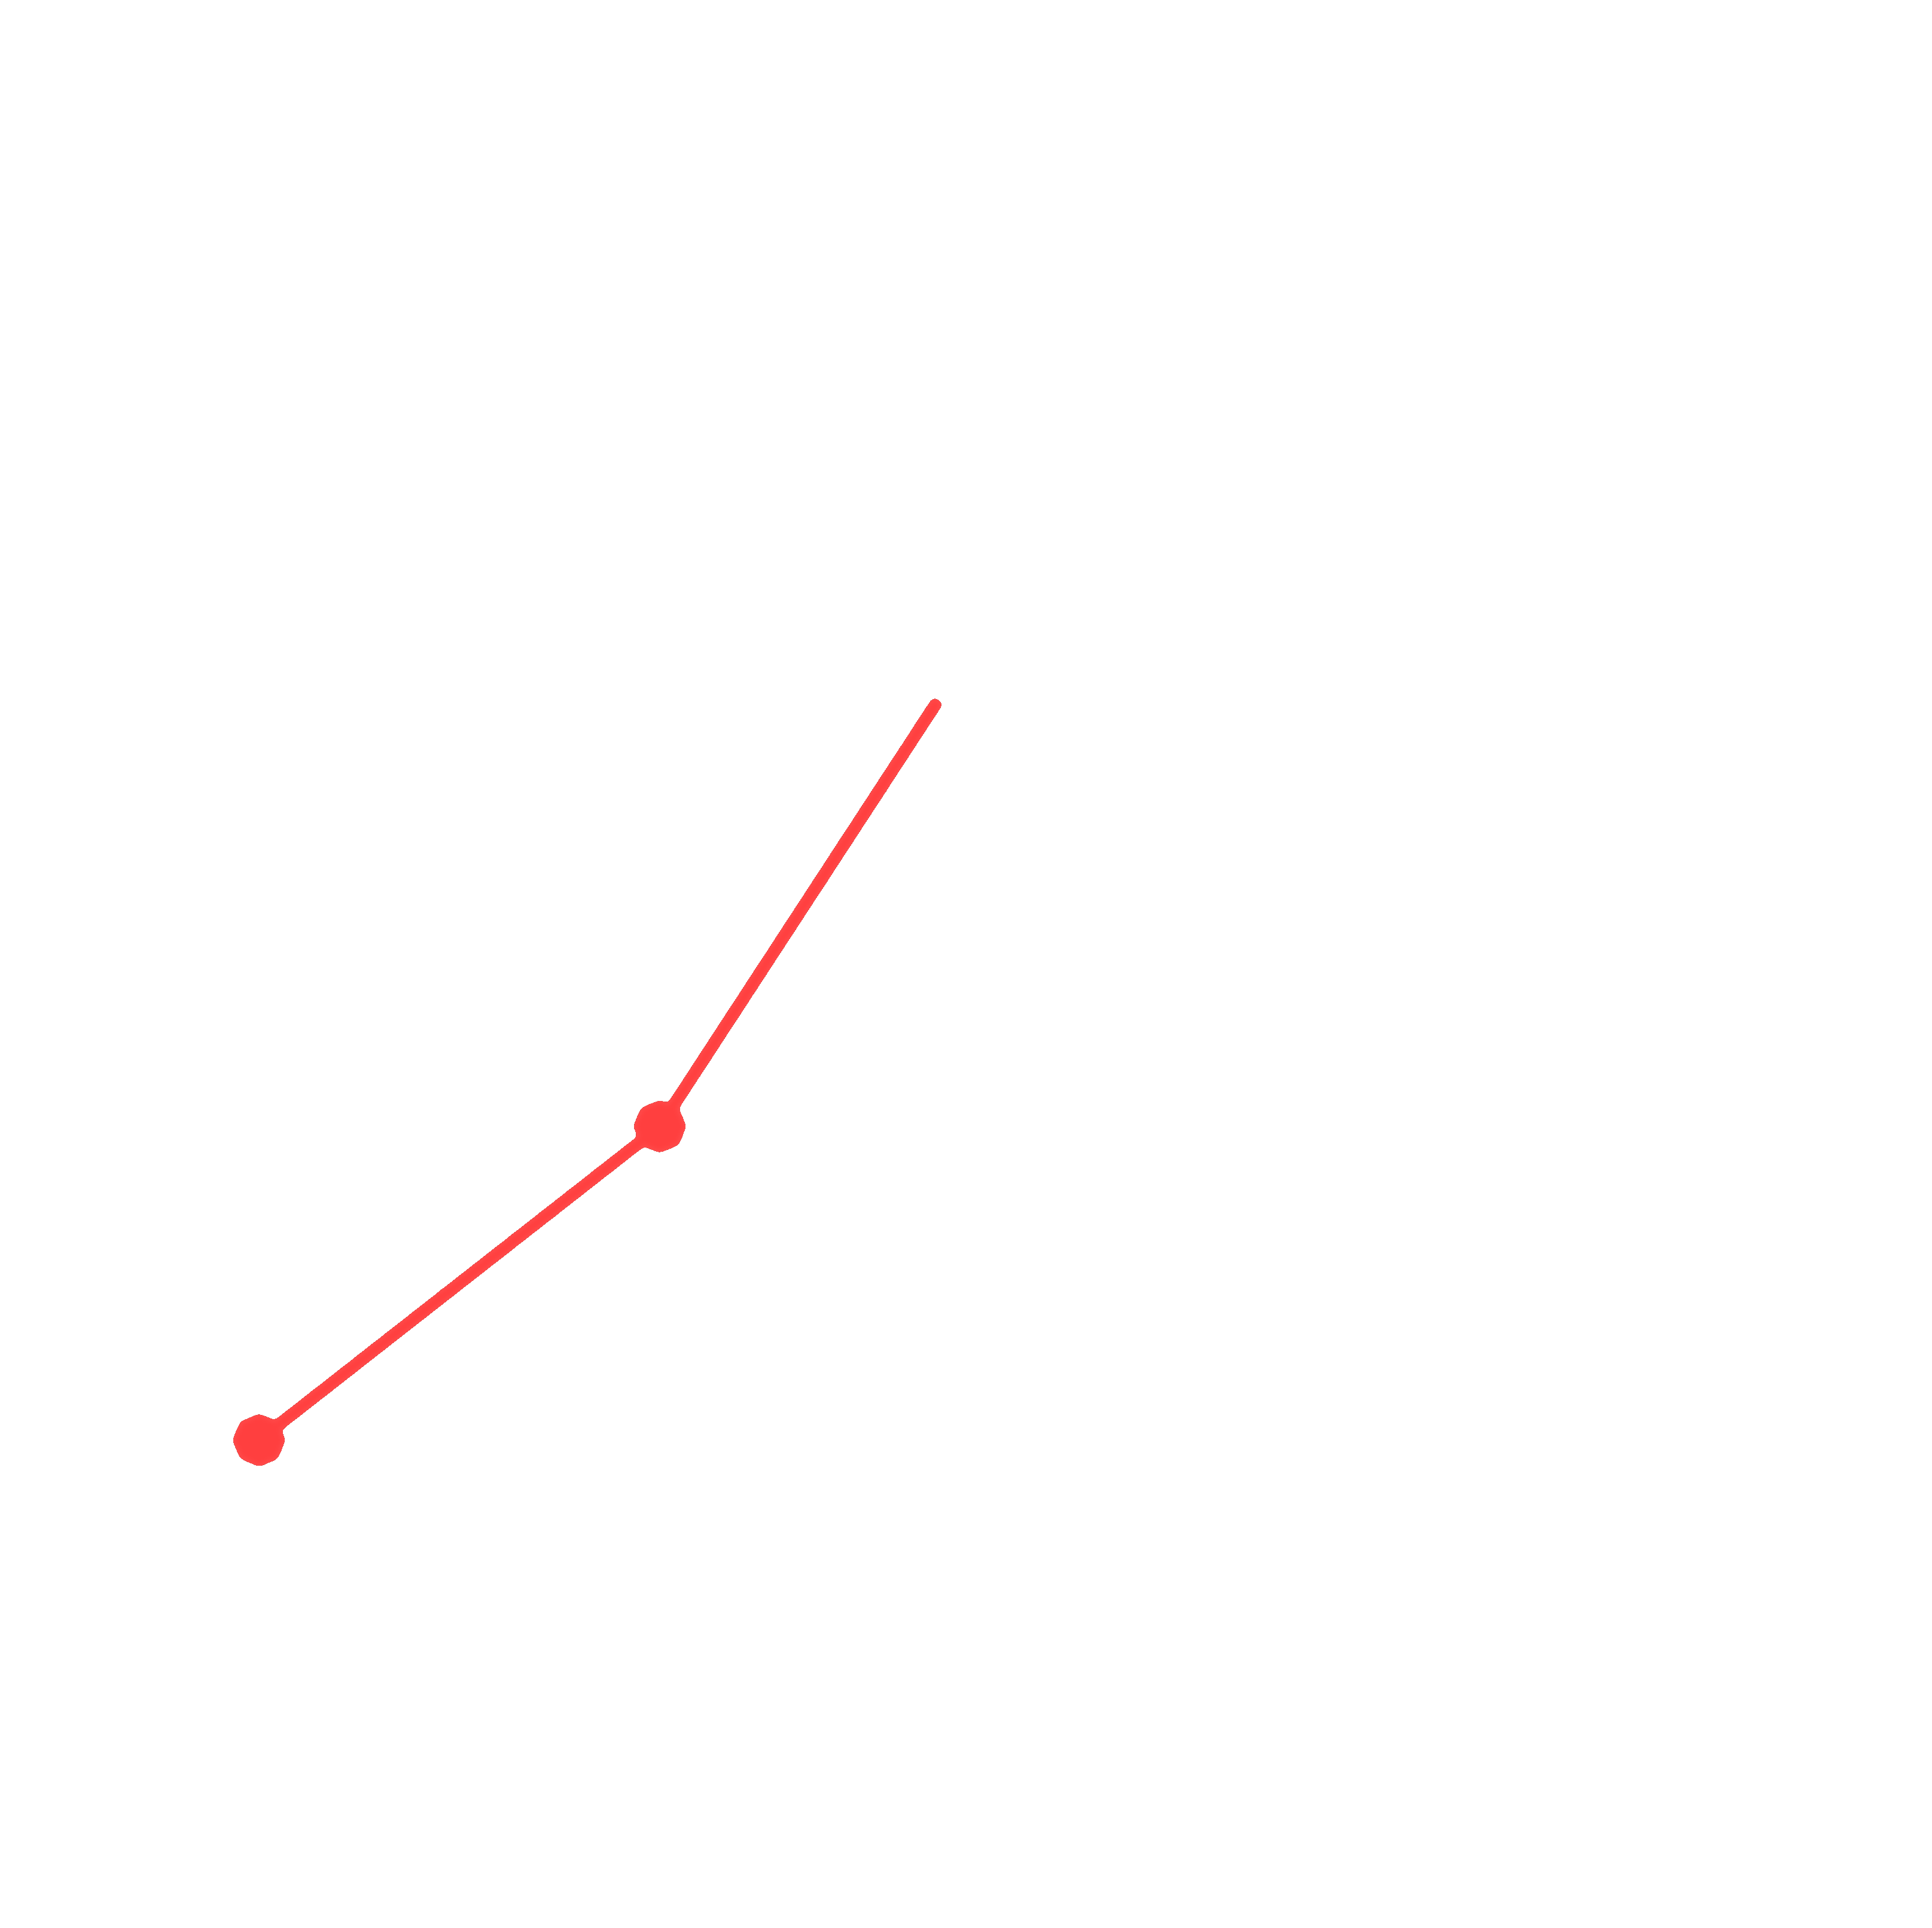
\includegraphics[width=\textwidth]{papers/doppelpendel/images/pendel_stand_nichtchaotisch.png}
    \end{minipage}
    \hfill
    \begin{minipage}{0.45\textwidth}
        \centering
        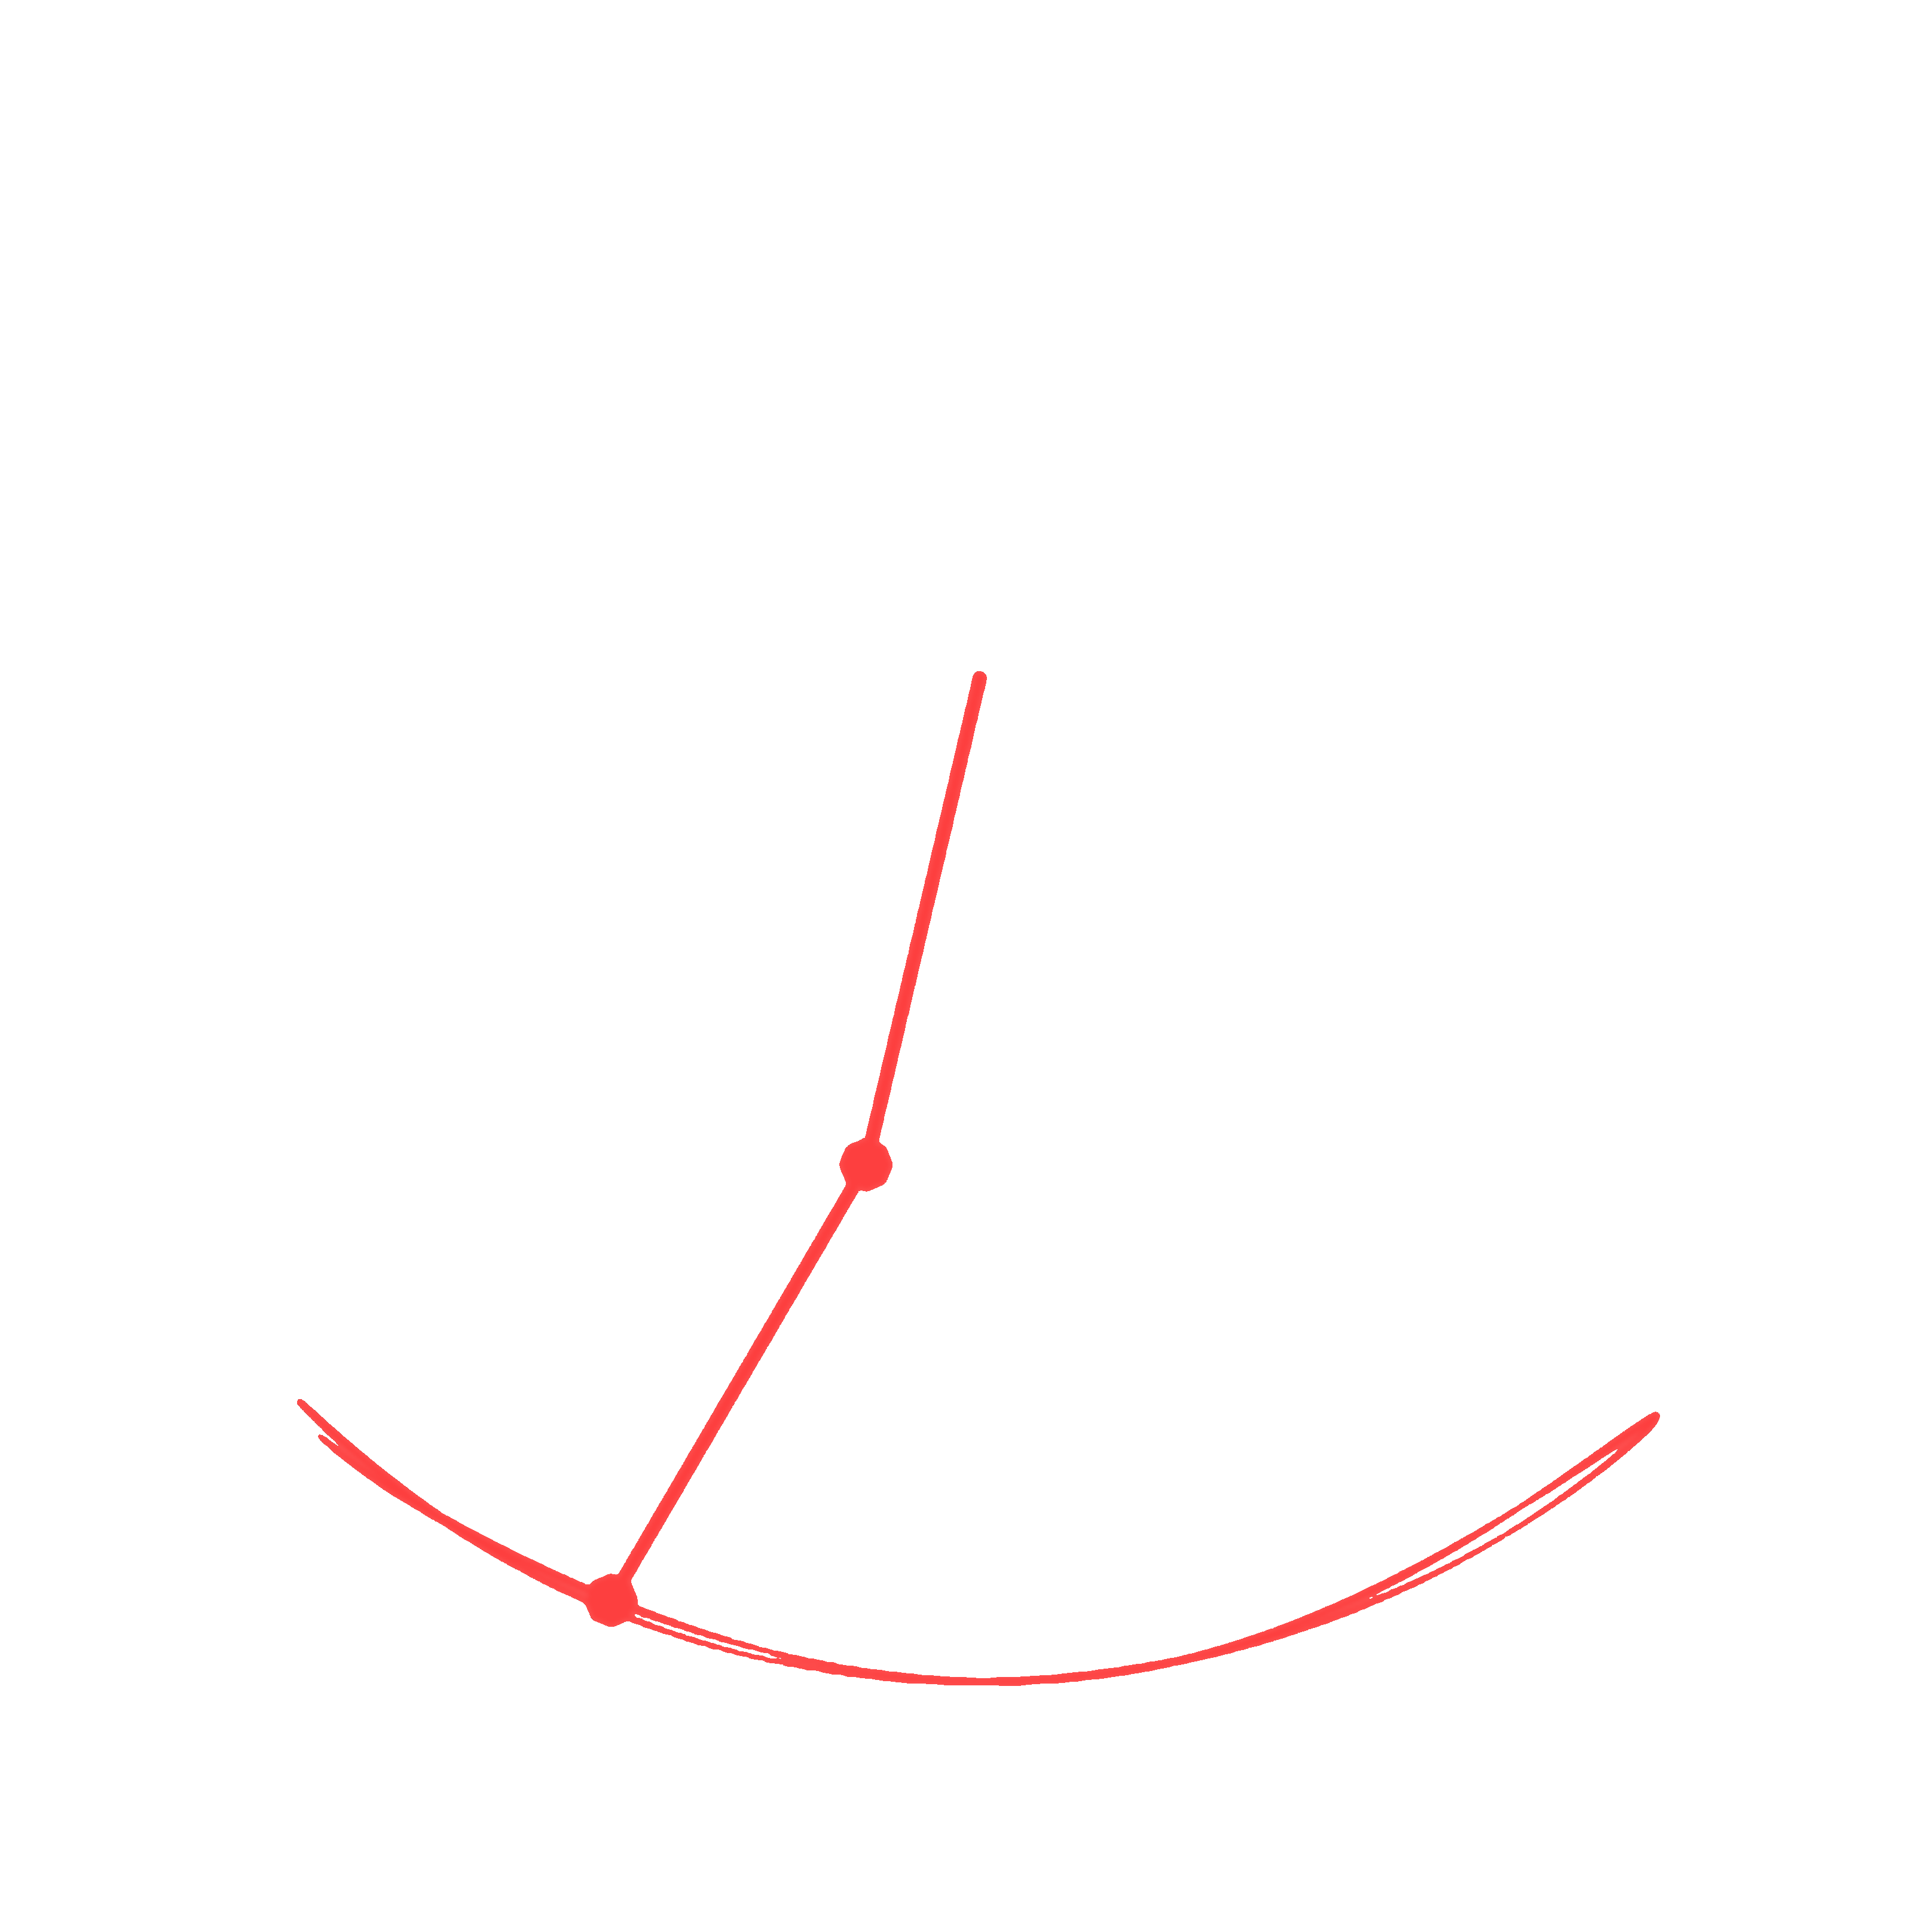
\includegraphics[width=\textwidth]{papers/doppelpendel/images/pendel_spur_nichtchaotisch.png}
    \end{minipage}
    \caption{Pendel wird nicht chaotisch, aufgrund kleiner Winkel.}
    \label{fig:pendel_nichtchaotisch}
\end{figure}

Was wir hier für drei verschiedene Anfangsbedingungen durchgeführt haben, kann man natürlich
für etliche Winkel durchrechnen lassen und beeurteilen ob bei gegebenem Winkel das System chaotisch wird.
Das wurde durch einen Schüler im <<Schweizer Jugend forscht>> mithilfe eines Programms untersucht.
Das Resultat wurde im sogenannten Parameterraum ausgegeben
ersichtlich in Abblildung \ref{fig:Parameterraum}.
\begin{figure}
    \centering
    \begin{minipage}{0.45\textwidth}
        \centering
        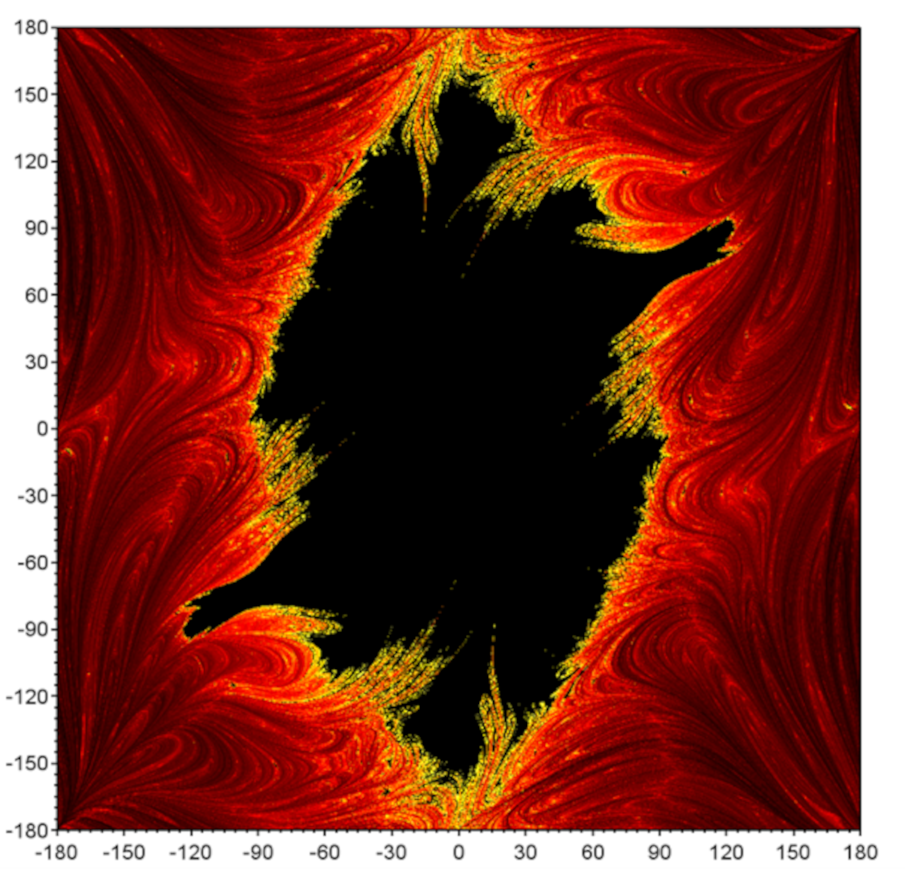
\includegraphics[width=\textwidth]{papers/doppelpendel/images/parameterraum.png}
    \end{minipage}
    \hfill
    \begin{minipage}{0.45\textwidth}
        \centering
        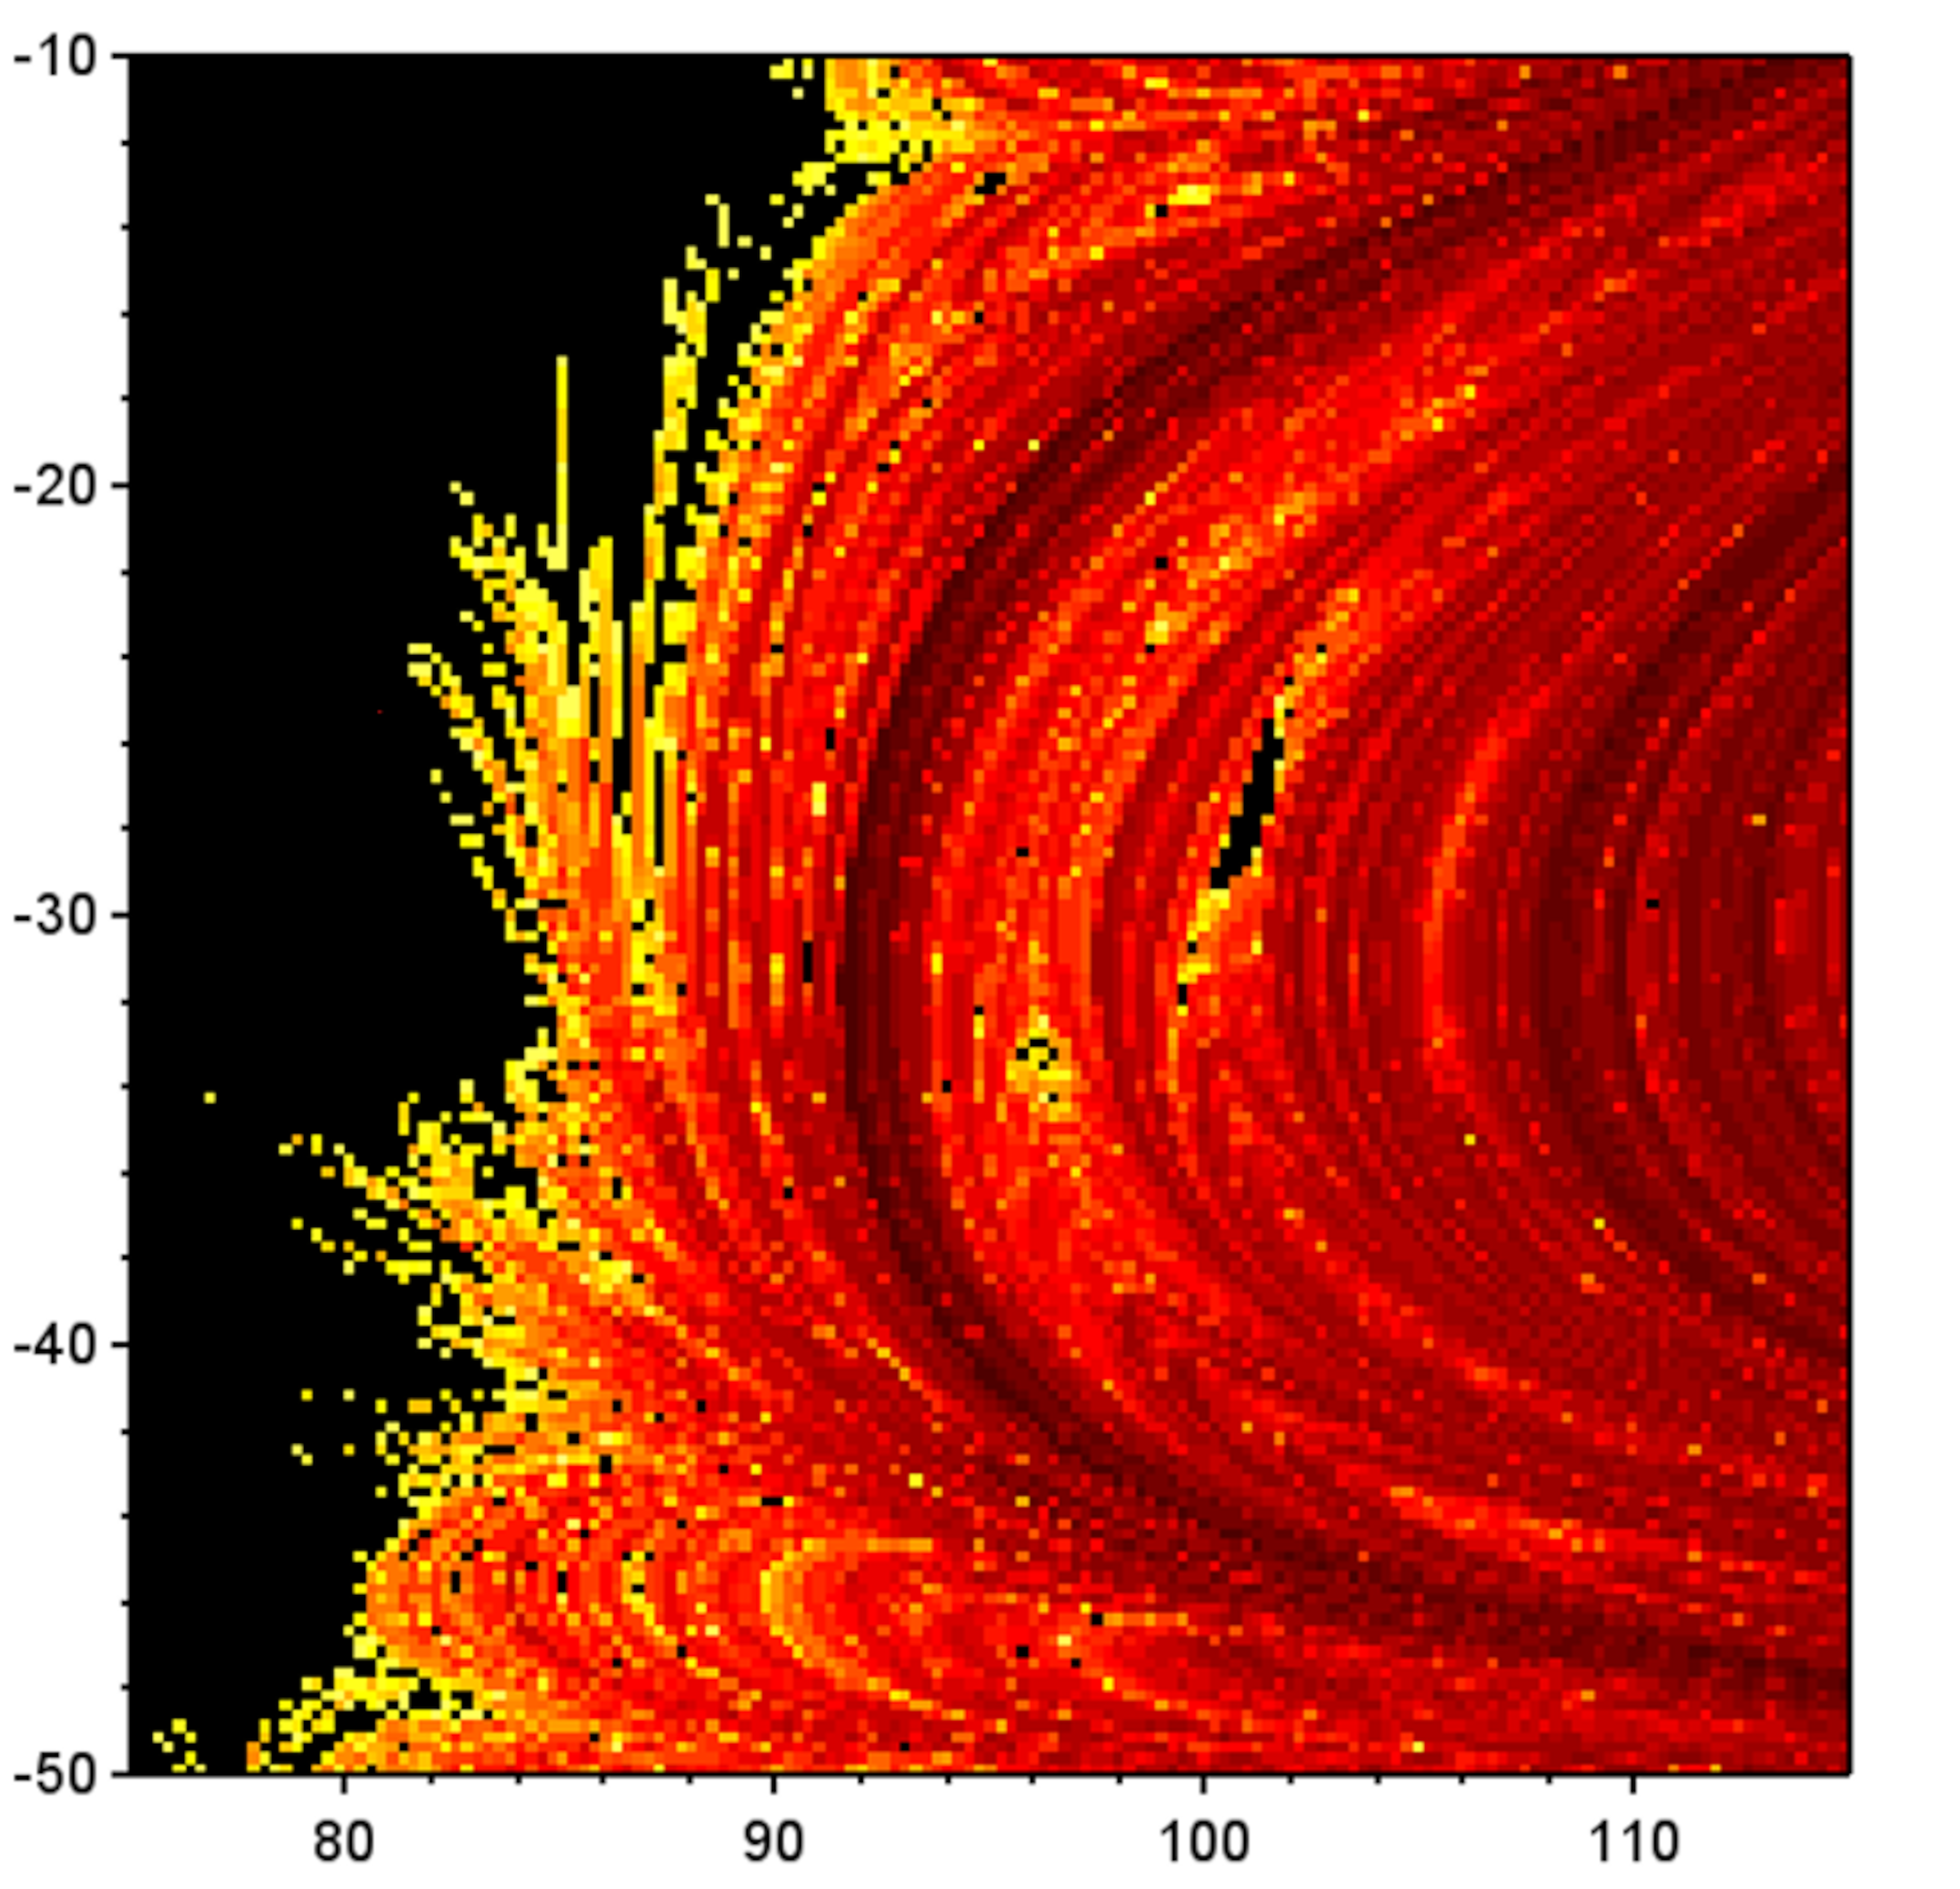
\includegraphics[width=\textwidth]{papers/doppelpendel/images/parameterraum_stabile_inseln.png}
    \end{minipage}
    \caption{Winkelpaare im Parameterraum (links) und stabile Inseln im Parameterraum (rechts)}
    \label{fig:Parameterraum}
\end{figure}
Auf der horizantalen Achse sind Anfangswinkel von \(\theta_1\) und
auf der vertikalen diejenigen von \(\theta_2\).
Schwarz bildet die Winkelpaare ab, die nicht ins Chaos übergehen.
Die farbigen Punkte sind daher kritische Winkelpaare.
Es wird unterschieden zwischen dunkelroten Punkten,
das sind Winkelpaare die schnell chaotisch werden, und
gelben Punkten, die eine kritische Zeit nah an 30 Sekunden haben. %Zitat Davide